\section{Uncertainty, multiplicity, and robustness}
\label{app:inference}

\subsection{Primary sampling unit and estimands}
All version contrasts are paired within country. We first average the five generations
within each country--question--model cell, then aggregate questions as required by the
metric. The 64 countries are the resampling and randomization units. Treating 3,840
responses as independent would be anti-conservative because five generations share the
same model, prompt, country, and survey target.

For every model estimate and version contrast, we report a point estimate,
country-cluster bootstrap standard error, and 95\% bias-corrected and accelerated (BCa)
interval from 20,000 resamples. A paired sign-flip randomization test with 19,999 draws
tests whether the country-level contrast is centered at zero; Monte Carlo standard errors
are released for every randomization $p$-value. Holm correction spans the five global
target-loss contrasts.

The main item-level test is a single family containing six questions under W1 and TVD
(12 outcomes). Each permutation applies the same country sign to all outcomes, and the
maximum absolute studentized statistic controls familywise error. A country bootstrap
supplies simultaneous 95\% max-$T$ intervals. Legacy within-metric Holm values remain in
the result files for transparency but do not determine the paper's item claims.

\subsection{Why 20,000 bootstrap draws are computationally sufficient}
We reran percentile-interval diagnostics using the first 1,000, 5,000, 10,000, and
20,000 draws. From 10,000 to 20,000, the largest absolute endpoint movement is
$0.00027$ for W1, $0.00034$ for TVD, $0.00226$ for CRG, $0.00082$ for VDR, and
$0.00228$ for CSR (Table~\ref{tab:bootstrap-convergence}). More draws would reduce
simulation noise but would not remove cross-country heterogeneity or unavailable
survey-design uncertainty.

\subsection{Three uncertainty sources}
The primary BCa intervals resample countries. Two 5,000-draw conditional sensitivities
ask narrower questions: how estimates vary when unweighted human cell counts are redrawn
multinomially, and how they vary when the five model generations are resampled within
cells. Both hold countries fixed. Figure~\ref{fig:uncertainty} shows that their W1/TVD
intervals are much narrower than the country bootstrap; country heterogeneity, rather
than too few random draws, dominates the remaining uncertainty.

\begin{figure}[h]
\centering
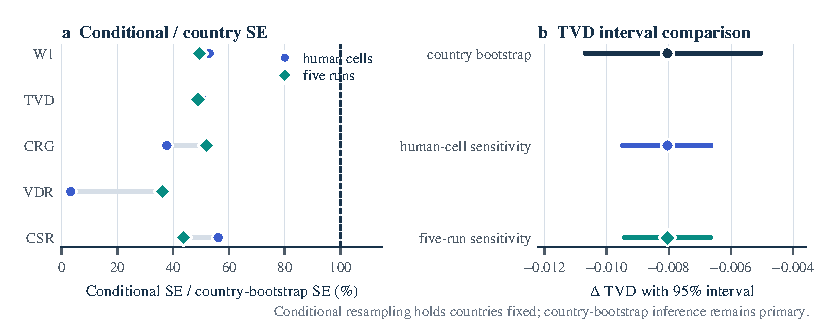
\includegraphics[width=\linewidth]{figs/figS1_uncertainty_sources.pdf}
\caption{Separating uncertainty sources. \textbf{a}, Conditional standard errors from
5,000 human-cell and five-run resamples, shown as percentages of the corresponding
country-bootstrap standard error; the dashed line marks equality. \textbf{b}, The
global TVD contrast under country-bootstrap, human-cell, and five-run 95\% intervals.
Conditional sensitivities hold countries fixed and complement rather than replace
country-cluster inference.}
\label{fig:uncertainty}
\end{figure}

\subsection{Prompt, composition, and influence checks}
The five-anchor analysis excludes Q121. Additional bounds move 50\% or 100\% of each
model's category-1 mass to category 2 before rescoring; they bound the internal label
conflict but cannot recreate a corrected generation.

For $K=1,\ldots,5$, the composition analysis exhaustively averages every subset of the
five observed generations. It uses no synthetic agents and makes no independence claim
about generations. The finite-population identity in Section 2 holds to machine precision
for every country--item cell. Country bootstrap intervals and paired sign flips again use
64 inferential units.

Finally, we recompute global W1 and TVD after omitting each of eight descriptive cultural
regions and within quartiles of average human-cell size. These are influence checks, not
new target populations. Cell-size ties yield quartile counts of 17, 15, 16, and 16.
Complete values appear in Appendix~\ref{app:results}.

\begin{figure}[h]
\centering
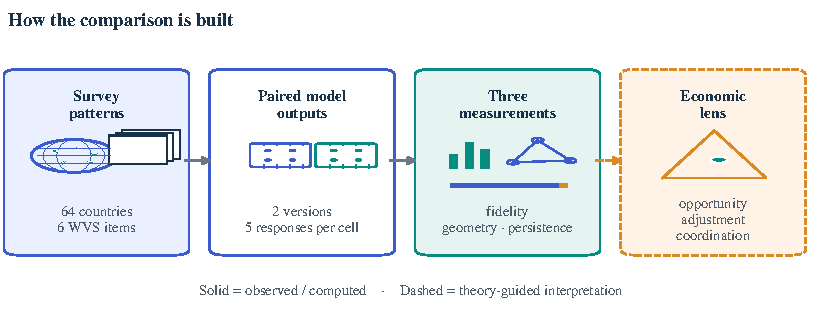
\includegraphics[width=\linewidth]{figs/figS2_study_design.pdf}
\caption{How the comparison is built. Solid boxes and arrows trace the released survey
distributions, paired model outputs, and computed fidelity, geometry, and persistence
measurements. The dashed final path is a theory-guided economic interpretation, not an
estimated welfare or policy effect.}
\label{fig:design}
\end{figure}
\FloatBarrier
